\documentclass[dvipsnames, tikz]{standalone}
\usepackage{amsmath}
\usepackage{arevmath}
\usepackage{xcolor}
\usepackage{tikz}
\usetikzlibrary{calc}
\usetikzlibrary{decorations.pathreplacing,calligraphy,3d}
\usetikzlibrary{matrix,shapes,fit,backgrounds}

\begin{document}
	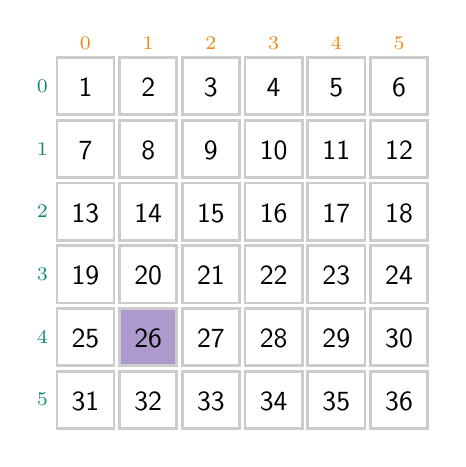
\begin{tikzpicture}[
		%Global config
		>=latex,
		line width=1pt,
		color = black,
		every left delimiter/.style={xshift=1ex},
		every right delimiter/.style={xshift=-1ex},
		%Styles
		Vector/.style={
			matrix of nodes,
			text height=2.5ex,
			text depth=0.75ex,
			text width=3.25ex,
			align=center,
			%left delimiter=(,
			%right delimiter=),
			column sep=1pt,
			row sep=1pt,
			nodes={draw=black!20}, % Uncoment to see the square nodes.
			%nodes in empty cells,
		},
		Matrix/.style={
			matrix of nodes,
			%text height=2.5ex,
			%text depth=0.75ex,
			%text width=3.25ex,
			%align=center,
			left delimiter=(,
			right delimiter=),
			%column sep=1pt,
			%row sep=1pt,
			%nodes={draw=black!10}, % Uncoment to see the square nodes.
			%nodes in empty cells,
		},
		DA/.style={
			fill,
			opacity=0.5,
			%rounded corners,
			inner sep=-1pt,
			line width=1pt,
		},
		DG/.style={
			line cap = round,
			rounded corners=0.25ex,
			line width = 8pt,
			opacity = 0.3,
		}
		]
		
		\matrix[Vector] at (0,0) (M){ % Matrix contents  
			\sf 1 & \sf 2 & \sf 3 & \sf 4 & \sf 5 & \sf 6\\
			\sf 7 & \sf 8 & \sf 9 & \sf 10 & \sf 11 & \sf 12\\
			\sf 13 & \sf 14 & \sf 15 & \sf 16 & \sf 17 & \sf 18\\
			\sf 19 & \sf 20 & \sf 21 & \sf 22 & \sf 23 & \sf 24\\
			\sf 25 & \sf 26 & \sf 27 & \sf 28 & \sf 29 & \sf 30\\
			\sf 31 & \sf 32 & \sf 33 & \sf 34 & \sf 35 & \sf 36\\
		};
		
		\begin{scope}[on background layer, font=\scriptsize]
			%To delimit internal area groups
			\node[DA,RoyalPurple,fit=(M-5-2)(M-5-2)](subM-2){};
			%\node[DA,green,fit=(M-6-4)(M-7-6)](subM-3){};
			
			% For line sectors
			%\draw[DG,LimeGreen](N-2-1.center) -- (N-2-2.center) -- (N-1-2.center)  (N-3-2.center)-- (N-2-2.center)-- (N-2-3.center); 
			\draw[PineGreen] (M-1-1.west) node[xshift=-1.1ex] {$0$};
			\draw[PineGreen] (M-2-1.west) node[xshift=-1.1ex] {$1$};
			\draw[PineGreen] (M-3-1.west) node[xshift=-1.1ex] {$2$};
			\draw[PineGreen] (M-4-1.west) node[xshift=-1.1ex] {$3$};
			\draw[PineGreen] (M-5-1.west) node[xshift=-1.1ex] {$4$};
			\draw[PineGreen] (M-6-1.west) node[xshift=-1.1ex] {$5$};
			
			\draw[BurntOrange] (M-1-1.north) node[yshift=1.1ex] {$0$};
			\draw[BurntOrange] (M-1-2.north) node[yshift=1.1ex] {$1$};
			\draw[BurntOrange] (M-1-3.north) node[yshift=1.1ex] {$2$};
			\draw[BurntOrange] (M-1-4.north) node[yshift=1.1ex] {$3$};
			\draw[BurntOrange] (M-1-5.north) node[yshift=1.1ex] {$4$};
			\draw[BurntOrange] (M-1-6.north) node[yshift=1.1ex] {$5$};
		\end{scope}
		
	\end{tikzpicture}
\end{document}